% !TEX root = main.tex
\subsection{Noise measurement}
\label{sec:Noisemeasurement}
The first step in the EFNMR Remote experiment is to measure the external noise.
The external noise depends on the location where the setup is placed, the orientation of the probe and on surrounding metal objects e.g. a metal desk.
To detect this external noise, a measurement without an NMR signal is provided.
The time domain noise signal is shown in figure \ref{fig: noise}.
It is clearly visible that the noise is centered around \SI{0}{\mu \volt}.
To gain knowledge about the noise level, the computer calculates the root-mean-square (RMS).
This means that it calculates the square of each data point, then sums up all the squared values, calculates the average and then applies a square root.
With this method the noise level can be calculated.
In this case it has a value of \SI{7.5}{\mu \volt}.
This is of an acceptable magnitude because any value below \SI{10}{\mu \volt} is good enough to provide meaningful NMR data.

\begin{figure}[H]
    \centering
    % GNUPLOT: LaTeX picture with Postscript
\begingroup
  % Encoding inside the plot.  In the header of your document, this encoding
  % should to defined, e.g., by using
  % \usepackage[cp1252,<other encodings>]{inputenc}
  \inputencoding{cp1252}%
  \makeatletter
  \providecommand\color[2][]{%
    \GenericError{(gnuplot) \space\space\space\@spaces}{%
      Package color not loaded in conjunction with
      terminal option `colourtext'%
    }{See the gnuplot documentation for explanation.%
    }{Either use 'blacktext' in gnuplot or load the package
      color.sty in LaTeX.}%
    \renewcommand\color[2][]{}%
  }%
  \providecommand\includegraphics[2][]{%
    \GenericError{(gnuplot) \space\space\space\@spaces}{%
      Package graphicx or graphics not loaded%
    }{See the gnuplot documentation for explanation.%
    }{The gnuplot epslatex terminal needs graphicx.sty or graphics.sty.}%
    \renewcommand\includegraphics[2][]{}%
  }%
  \providecommand\rotatebox[2]{#2}%
  \@ifundefined{ifGPcolor}{%
    \newif\ifGPcolor
    \GPcolorfalse
  }{}%
  \@ifundefined{ifGPblacktext}{%
    \newif\ifGPblacktext
    \GPblacktexttrue
  }{}%
  % define a \g@addto@macro without @ in the name:
  \let\gplgaddtomacro\g@addto@macro
  % define empty templates for all commands taking text:
  \gdef\gplbacktext{}%
  \gdef\gplfronttext{}%
  \makeatother
  \ifGPblacktext
    % no textcolor at all
    \def\colorrgb#1{}%
    \def\colorgray#1{}%
  \else
    % gray or color?
    \ifGPcolor
      \def\colorrgb#1{\color[rgb]{#1}}%
      \def\colorgray#1{\color[gray]{#1}}%
      \expandafter\def\csname LTw\endcsname{\color{white}}%
      \expandafter\def\csname LTb\endcsname{\color{black}}%
      \expandafter\def\csname LTa\endcsname{\color{black}}%
      \expandafter\def\csname LT0\endcsname{\color[rgb]{1,0,0}}%
      \expandafter\def\csname LT1\endcsname{\color[rgb]{0,1,0}}%
      \expandafter\def\csname LT2\endcsname{\color[rgb]{0,0,1}}%
      \expandafter\def\csname LT3\endcsname{\color[rgb]{1,0,1}}%
      \expandafter\def\csname LT4\endcsname{\color[rgb]{0,1,1}}%
      \expandafter\def\csname LT5\endcsname{\color[rgb]{1,1,0}}%
      \expandafter\def\csname LT6\endcsname{\color[rgb]{0,0,0}}%
      \expandafter\def\csname LT7\endcsname{\color[rgb]{1,0.3,0}}%
      \expandafter\def\csname LT8\endcsname{\color[rgb]{0.5,0.5,0.5}}%
    \else
      % gray
      \def\colorrgb#1{\color{black}}%
      \def\colorgray#1{\color[gray]{#1}}%
      \expandafter\def\csname LTw\endcsname{\color{white}}%
      \expandafter\def\csname LTb\endcsname{\color{black}}%
      \expandafter\def\csname LTa\endcsname{\color{black}}%
      \expandafter\def\csname LT0\endcsname{\color{black}}%
      \expandafter\def\csname LT1\endcsname{\color{black}}%
      \expandafter\def\csname LT2\endcsname{\color{black}}%
      \expandafter\def\csname LT3\endcsname{\color{black}}%
      \expandafter\def\csname LT4\endcsname{\color{black}}%
      \expandafter\def\csname LT5\endcsname{\color{black}}%
      \expandafter\def\csname LT6\endcsname{\color{black}}%
      \expandafter\def\csname LT7\endcsname{\color{black}}%
      \expandafter\def\csname LT8\endcsname{\color{black}}%
    \fi
  \fi
    \setlength{\unitlength}{0.0500bp}%
    \ifx\gptboxheight\undefined%
      \newlength{\gptboxheight}%
      \newlength{\gptboxwidth}%
      \newsavebox{\gptboxtext}%
    \fi%
    \setlength{\fboxrule}{0.5pt}%
    \setlength{\fboxsep}{1pt}%
\begin{picture}(7200.00,5040.00)%
    \gplgaddtomacro\gplbacktext{%
      \csname LTb\endcsname%%
      \put(814,704){\makebox(0,0)[r]{\strut{}$-80$}}%
      \put(814,1218){\makebox(0,0)[r]{\strut{}$-60$}}%
      \put(814,1733){\makebox(0,0)[r]{\strut{}$-40$}}%
      \put(814,2247){\makebox(0,0)[r]{\strut{}$-20$}}%
      \put(814,2762){\makebox(0,0)[r]{\strut{}$0$}}%
      \put(814,3276){\makebox(0,0)[r]{\strut{}$20$}}%
      \put(814,3790){\makebox(0,0)[r]{\strut{}$40$}}%
      \put(814,4305){\makebox(0,0)[r]{\strut{}$60$}}%
      \put(814,4819){\makebox(0,0)[r]{\strut{}$80$}}%
      \put(946,484){\makebox(0,0){\strut{}$0$}}%
      \put(1727,484){\makebox(0,0){\strut{}$0.2$}}%
      \put(2508,484){\makebox(0,0){\strut{}$0.4$}}%
      \put(3289,484){\makebox(0,0){\strut{}$0.6$}}%
      \put(4070,484){\makebox(0,0){\strut{}$0.8$}}%
      \put(4851,484){\makebox(0,0){\strut{}$1$}}%
      \put(5632,484){\makebox(0,0){\strut{}$1.2$}}%
      \put(6413,484){\makebox(0,0){\strut{}$1.4$}}%
    }%
    \gplgaddtomacro\gplfronttext{%
      \csname LTb\endcsname%%
      \put(209,2761){\rotatebox{-270}{\makebox(0,0){\strut{}Amplitude in $\si{\mu \volt}$}}}%
      \put(3874,154){\makebox(0,0){\strut{}Time in $\si{\second}$}}%
      \csname LTb\endcsname%%
      \put(5816,4646){\makebox(0,0)[r]{\strut{}noise signal}}%
    }%
    \gplbacktext
    \put(0,0){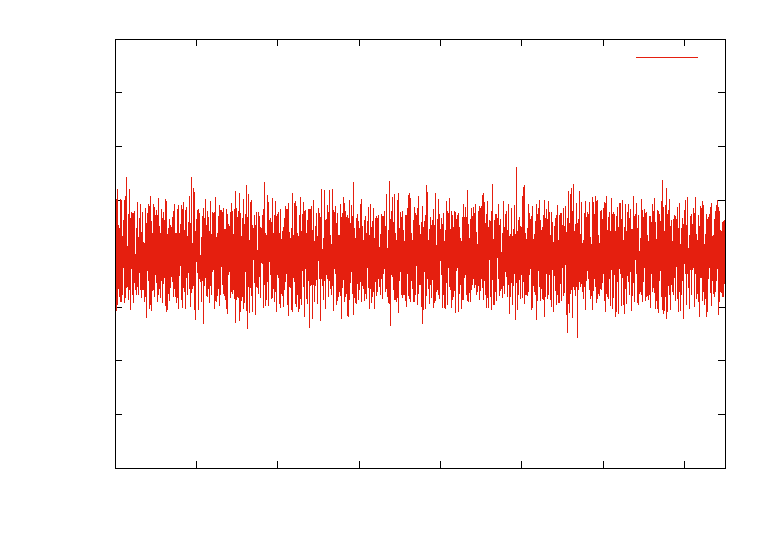
\includegraphics{plots/noise}}%
    \gplfronttext
  \end{picture}%
\endgroup

    \caption[Noise signal taken by the B$_1$ coil.]{Noise signal taken by the B$_1$ coil.
    The noise value of this signal is \SI{7.5}{\mu \volt}.}
    \label{fig: noise}
\end{figure}

Figure \ref{fig: MonitorNoise138} shows the frequency domain noise.
This means that the time domain is fourier transformed into the frequency domain.
This method is one of the basic principles used in this experiment to make research about the properties of the measured signals.
The frequency domain noise shows very specific sharp peaks every \SI{50}{\hertz} interval.
To be more precise the peaks in the middle of every hundred \si{\hertz} step are way higher than those at \SI{1400}{\hertz}, \SI{1500}{\hertz} and so on.
This results from the frequency in the power grid which is \SI{50}{\hertz} in Germany and can also be affiliated to the electrical noise of a surrounding fluorescent light or the CRT computer monitor.
Unfortunately the remote camera program of the computer did not work and therefore it is not clear if there was a fluorescent light in the room.
Even though the noise peaks in the frequency domain figure \ref{fig: MonitorNoise138} indicate that there could be a fluorescent light source in the room.
Despite all sharp peaks, there is also a slight increase of the amplitude around $\SI{185 \pm 10 e1}{\frac{\mu \volt}{\hertz}}$ visible.
This is explicable by the resonance frequency of the instrument and its sensitvity around the larmor frequency (\SI{1841.4}{\hertz} for water in Germany in July 2020).
All our following measurements will be done nearby the larmor frequency.
That is the reason why the instrument sensitvity is sharpend around this value.

\begin{figure}[H]
    \centering
    % GNUPLOT: LaTeX picture with Postscript
\begingroup
  % Encoding inside the plot.  In the header of your document, this encoding
  % should to defined, e.g., by using
  % \usepackage[cp1252,<other encodings>]{inputenc}
  \inputencoding{cp1252}%
  \makeatletter
  \providecommand\color[2][]{%
    \GenericError{(gnuplot) \space\space\space\@spaces}{%
      Package color not loaded in conjunction with
      terminal option `colourtext'%
    }{See the gnuplot documentation for explanation.%
    }{Either use 'blacktext' in gnuplot or load the package
      color.sty in LaTeX.}%
    \renewcommand\color[2][]{}%
  }%
  \providecommand\includegraphics[2][]{%
    \GenericError{(gnuplot) \space\space\space\@spaces}{%
      Package graphicx or graphics not loaded%
    }{See the gnuplot documentation for explanation.%
    }{The gnuplot epslatex terminal needs graphicx.sty or graphics.sty.}%
    \renewcommand\includegraphics[2][]{}%
  }%
  \providecommand\rotatebox[2]{#2}%
  \@ifundefined{ifGPcolor}{%
    \newif\ifGPcolor
    \GPcolorfalse
  }{}%
  \@ifundefined{ifGPblacktext}{%
    \newif\ifGPblacktext
    \GPblacktexttrue
  }{}%
  % define a \g@addto@macro without @ in the name:
  \let\gplgaddtomacro\g@addto@macro
  % define empty templates for all commands taking text:
  \gdef\gplbacktext{}%
  \gdef\gplfronttext{}%
  \makeatother
  \ifGPblacktext
    % no textcolor at all
    \def\colorrgb#1{}%
    \def\colorgray#1{}%
  \else
    % gray or color?
    \ifGPcolor
      \def\colorrgb#1{\color[rgb]{#1}}%
      \def\colorgray#1{\color[gray]{#1}}%
      \expandafter\def\csname LTw\endcsname{\color{white}}%
      \expandafter\def\csname LTb\endcsname{\color{black}}%
      \expandafter\def\csname LTa\endcsname{\color{black}}%
      \expandafter\def\csname LT0\endcsname{\color[rgb]{1,0,0}}%
      \expandafter\def\csname LT1\endcsname{\color[rgb]{0,1,0}}%
      \expandafter\def\csname LT2\endcsname{\color[rgb]{0,0,1}}%
      \expandafter\def\csname LT3\endcsname{\color[rgb]{1,0,1}}%
      \expandafter\def\csname LT4\endcsname{\color[rgb]{0,1,1}}%
      \expandafter\def\csname LT5\endcsname{\color[rgb]{1,1,0}}%
      \expandafter\def\csname LT6\endcsname{\color[rgb]{0,0,0}}%
      \expandafter\def\csname LT7\endcsname{\color[rgb]{1,0.3,0}}%
      \expandafter\def\csname LT8\endcsname{\color[rgb]{0.5,0.5,0.5}}%
    \else
      % gray
      \def\colorrgb#1{\color{black}}%
      \def\colorgray#1{\color[gray]{#1}}%
      \expandafter\def\csname LTw\endcsname{\color{white}}%
      \expandafter\def\csname LTb\endcsname{\color{black}}%
      \expandafter\def\csname LTa\endcsname{\color{black}}%
      \expandafter\def\csname LT0\endcsname{\color{black}}%
      \expandafter\def\csname LT1\endcsname{\color{black}}%
      \expandafter\def\csname LT2\endcsname{\color{black}}%
      \expandafter\def\csname LT3\endcsname{\color{black}}%
      \expandafter\def\csname LT4\endcsname{\color{black}}%
      \expandafter\def\csname LT5\endcsname{\color{black}}%
      \expandafter\def\csname LT6\endcsname{\color{black}}%
      \expandafter\def\csname LT7\endcsname{\color{black}}%
      \expandafter\def\csname LT8\endcsname{\color{black}}%
    \fi
  \fi
    \setlength{\unitlength}{0.0500bp}%
    \ifx\gptboxheight\undefined%
      \newlength{\gptboxheight}%
      \newlength{\gptboxwidth}%
      \newsavebox{\gptboxtext}%
    \fi%
    \setlength{\fboxrule}{0.5pt}%
    \setlength{\fboxsep}{1pt}%
\begin{picture}(7200.00,5040.00)%
    \gplgaddtomacro\gplbacktext{%
      \csname LTb\endcsname%%
      \put(682,704){\makebox(0,0)[r]{\strut{}$0$}}%
      \put(682,1390){\makebox(0,0)[r]{\strut{}$2$}}%
      \put(682,2076){\makebox(0,0)[r]{\strut{}$4$}}%
      \put(682,2762){\makebox(0,0)[r]{\strut{}$6$}}%
      \put(682,3447){\makebox(0,0)[r]{\strut{}$8$}}%
      \put(682,4133){\makebox(0,0)[r]{\strut{}$10$}}%
      \put(682,4819){\makebox(0,0)[r]{\strut{}$12$}}%
      \put(814,484){\makebox(0,0){\strut{}$1400$}}%
      \put(1479,484){\makebox(0,0){\strut{}$1500$}}%
      \put(2145,484){\makebox(0,0){\strut{}$1600$}}%
      \put(2810,484){\makebox(0,0){\strut{}$1700$}}%
      \put(3476,484){\makebox(0,0){\strut{}$1800$}}%
      \put(4141,484){\makebox(0,0){\strut{}$1900$}}%
      \put(4807,484){\makebox(0,0){\strut{}$2000$}}%
      \put(5472,484){\makebox(0,0){\strut{}$2100$}}%
      \put(6138,484){\makebox(0,0){\strut{}$2200$}}%
      \put(6803,484){\makebox(0,0){\strut{}$2300$}}%
    }%
    \gplgaddtomacro\gplfronttext{%
      \csname LTb\endcsname%%
      \put(308,2761){\rotatebox{-270}{\makebox(0,0){\strut{}Amplitude in $\si{\frac{\mu \volt}{\hertz}}$}}}%
      \put(3808,154){\makebox(0,0){\strut{}Frequency in $\si{\hertz}$}}%
      \csname LTb\endcsname%%
      \put(5816,4646){\makebox(0,0)[r]{\strut{}noise magnitude spectrum}}%
    }%
    \gplbacktext
    \put(0,0){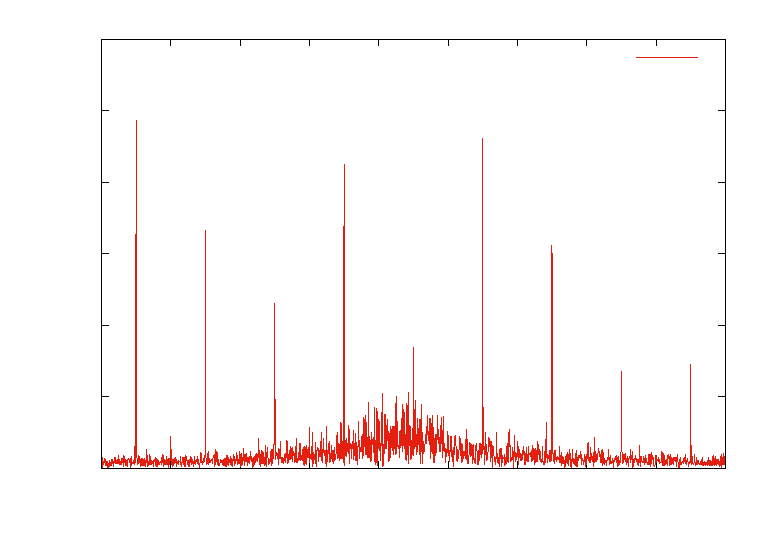
\includegraphics{plots/MonitorNoise138}}%
    \gplfronttext
  \end{picture}%
\endgroup

    \caption[Fourier transformed noise signal of the previous figure \ref{fig: noise}.]{Fourier transformed noise signal of the previous figure \ref{fig: noise}.
    Strong peaks every \SI{50}{\hertz} correspond to the frequency of the power grid in Germany and to electrical noise of a surrounding fluorescent light or the CRT computer monitor.
    The slight increase of the amplitude around $\SI{185 \pm 10}{\cdot 10^1 \frac{\mu \volt}{\hertz}}$ is explicable by the resonance frequency of instrument and its sensitvity around the larmor frequency (\SI{1841.4}{\hertz} for water in Germany in July 2020).}
    \label{fig: MonitorNoise138}
\end{figure}